\chapter{Objetivos del proyecto}

%\newpage
%Objetivos, alcance, planificación temporal, herramientas, 
%gestión de riesgos, evaluación económica

\section{Objetivos}
Los objetivos del proyecto consisten en crear un software que extienda la funcionalidad actual del sistema INTRASIM desarrollado 
por la universidad de Navarra y del grupo de investigación GALAN perteneciente a la UPV/EHU.

El software, permite cargar observaciones y propiedades previamente capturadas con diversas herramientas (Kinect) y
visualizarlas gr\'aficamente. Esas observaciones y propiedades se cargar\'an en un panel lateral con forma de \'arbol
y podr\'an seleccionarse para ser visualizadas. Los gr\'aficos pueden ser reorganizados como el
usuario quiera, para verlos al mismo tiempo.

La herramienta permite visualizar los datos en bruto y v\'{i}deo (si esta disponible). El fin de la herramienta es
permitir al usuario experto seleccionar un rango en cualquiera de los gr\'aficos y exportarlo en formato XML.

\section{Alcance}
El alcance del proyecto se define mediante una Estructura de Descomposición del Trabajo. Es una figura en la que de manera jer\'{a}rquica
se representa que es lo que va a hacerse.
\begin{figure}[H]
    \centering
    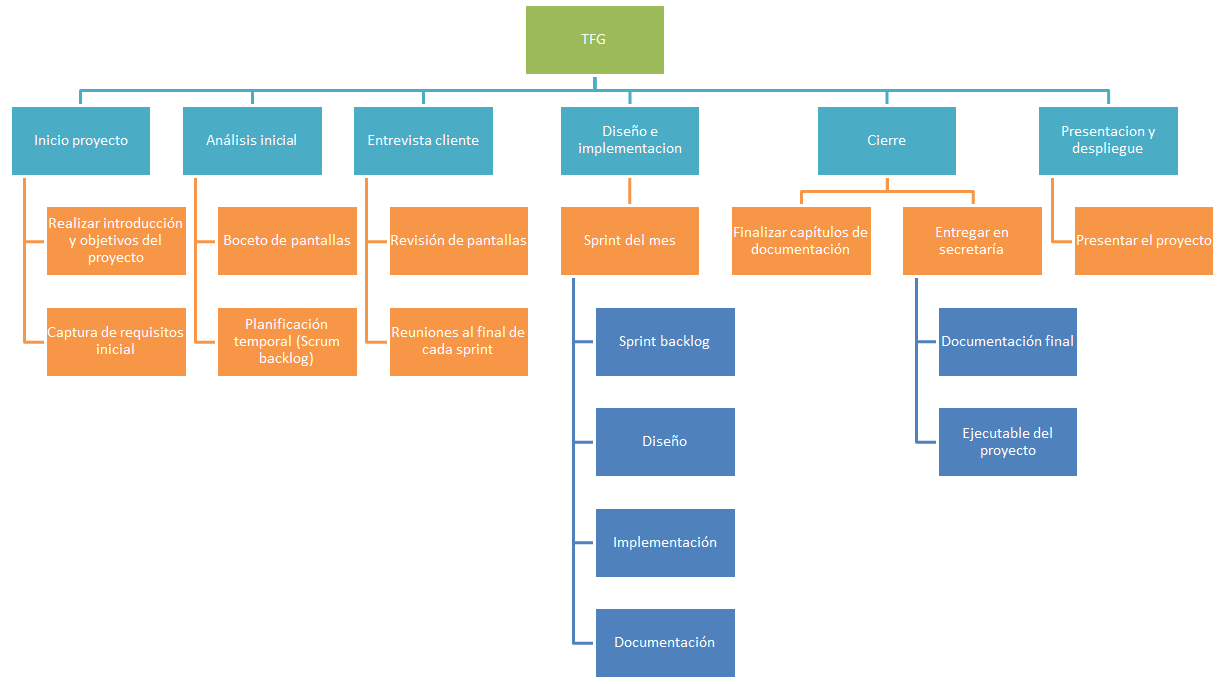
\includegraphics[width=1\linewidth]{./Figures/EDT}
    \caption[Alcance del proyecto]{EDT}
    \label{fig:Alcance}
\end{figure}

\subsection{An\'{a}lisis inicial}
\subsubsection{Boceto de pantallas}
\begin{table}[H]
    \begin{center}
        \rowcolors{1}{lightgray}{} %\rowcolors{<starting row index>}{<odd row color>}{<even row color>}
        \begin{tabular}{l p{8cm}}
            Responsable                           & Rub\'{e}n \\
            Duraci\'{o}n (horas)                  & 4. \\ 
            Esfuerzo (Horas / Persona)            & 2. \\
            Descripci\'{o}n                       & Diseño de pantallas inicial en base a las ideas obtenidas de lo
                                                    contado por Mikel, a fin de obtener dudas sobre funcionalidades. \\
            Entradas                              & Ninguna \\
            Salidas / Entregables                 & Boceto dibujado a mano con el dise\~{n}o de las pantallas \\
            Recursos necesarios                   & Papel y l\'{a}piz \\
            Precedencias                          & Ninguna \\
        \end{tabular}
    \end{center}
            
\end{table}

\subsubsection{Planificaci\'{o}n temporal (Scrum Backlog)}
\begin{table}[H]
    \begin{center}
        \rowcolors{1}{lightgray}{} %\rowcolors{<starting row index>}{<odd row color>}{<even row color>}
        \begin{tabular}{l p{8cm}}
            Responsable                           & Rub\'{e}n \\
            Duraci\'{o}n (horas)                  & 7. \\ 
            Esfuerzo (Horas / Persona)            & 7. \\
            Descripci\'{o}n                       & Creacion de cada sprint con sus respectivas tareas para crear la pila de tareas. \\
            Entradas                              & Requisitos del cliente.\\
            Salidas / Entregables                 & Un listado con todas las tareas a completar \\
            Recursos necesarios                   & PC con un editor de textos.\\
            Precedencias                          & Requisitos del cliente. \\
        \end{tabular}
    \end{center}
    
\end{table}

\subsubsection{Realizar introducci\'{o}n y objetivos del proyecto}
\begin{table}[H]
    \begin{center}
        \rowcolors{1}{lightgray}{} %\rowcolors{<starting row index>}{<odd row color>}{<even row color>}
        \begin{tabular}{l p{8cm}}
            Responsable                           & Rub\'{e}n \\
            Duraci\'{o}n                          & 7. \\ 
            Esfuerzo (Horas / Persona)            & 7. \\
            Descripci\'{o}n                       & Realizar las secciones de la memoria de la Introducci\'{o}n y los
                                                    objetivos del proyecto. \\
            Entradas                              & Scrum backlog  \\
            Salidas / Entregables                 & Los cap\'{i}tulos de introducci\'{o}n y objetivos del proyecto. \\
            Recursos necesarios                   & PC, \LaTeX, TeXStudio, Scrum backlog \\
            Precedencias                          & Scrum backlog. \\
        \end{tabular}
    \end{center}
    
\end{table}

\subsection{Entrevista cliente}
\subsubsection{Revisi\'{o}n de pantallas}
\begin{table}[H]
    \begin{center}
        \rowcolors{1}{lightgray}{} %\rowcolors{<starting row index>}{<odd row color>}{<even row color>}
        \begin{tabular}{l p{8cm}}
            Responsable                           & Rub\'{e}n \\
            Duraci\'{o}n                          & 2. \\ 
            Esfuerzo (Horas / Persona)            & 1.5 \\
            Descripci\'{o}n                       & Mostrar al cliente (Mikel), un prototipo inicial de pantallas
                                                    para asi poder mejorar el dise\~{n}o para que sea mas f\'{a}cil de usar. \\
            Entradas                              & Requisitos del cliente. \\
            Salidas / Entregables                 & Prototipo realizado en WPF que muestra el comportamiento y forma de las pantallas. \\
            Recursos necesarios                   & Visual Studio 2013, Avalon Dock, un PC. \\
            Precedencias                          & Captura de requisitos inicial. \\
        \end{tabular}
    \end{center}
    
\end{table}

\subsubsection{Reuniones al final de cada sprint}
\begin{table}[H]
    \begin{center}
        \rowcolors{1}{lightgray}{} %\rowcolors{<starting row index>}{<odd row color>}{<even row color>}
        \begin{tabular}{l p{8cm}}
            Responsable                           & Rub\'{e}n \\
            Duraci\'{o}n                          & 2. \\ 
            Esfuerzo (Horas / Persona)            & 1.5 \\
            Descripci\'{o}n                       & Reuni\'{o}n para que el director de proyecto vea como va el trabajo,
                                                    aclarar dudas etc. \\
            Entradas                              & El trabajo realizado hasta el momento.\\
            Salidas / Entregables                 & Ninguno / acta de reuni\'{o}n \\
            Recursos necesarios                   & PC con el programa funcional. \\
            Precedencias                          & Ninguno. \\
        \end{tabular}
    \end{center}
    
\end{table}

\subsection{Dise\~{n}o e implementaci\'{o}n}
\subsubsection{Sprint backlog}
\begin{table}[H]
    \begin{center}
        \rowcolors{1}{lightgray}{} %\rowcolors{<starting row index>}{<odd row color>}{<even row color>}
        \begin{tabular}{l p{8cm}}
            Responsable                           & Rub\'{e}n \\
            Duraci\'{o}n                          & 1 \\ 
            Esfuerzo (Horas / Persona)            & 0.5 \\
            Descripci\'{o}n                       & Elegir las tareas que van a conformar el sprint del mes. \\
            Entradas                              & La lista de tareas completa\\
            Salidas / Entregables                 & Post-it con las tareas seleccionadas para ese sprint \\
            Recursos necesarios                   & Post-it, boli y lista de tareas. \\
            Precedencias                          & Scrum backlog \\
        \end{tabular}
    \end{center}
    
\end{table}

\subsubsection{Dise\~{n}o}
\begin{table}[H]
    \begin{center}
        \rowcolors{1}{lightgray}{} %\rowcolors{<starting row index>}{<odd row color>}{<even row color>}
        \begin{tabular}{l p{8cm}}
            Responsable                           & Rub\'{e}n \\
            Duraci\'{o}n                          & 10. \\ 
            Esfuerzo (Horas / Persona)            & 4. \\
            Descripci\'{o}n                       & Realizar el diseño de software, clases, Interfaces necesarias, que patrones van a usarse etc. \\
            Entradas                              & Tarea a realizar y la interfaz de usuario.\\
            Salidas / Entregables                 & Dise\~{n}o de software que guiar\'{a} la siguiente tarea y la documentaci\'{o}n
                                                    habr\'{a} sido actualizada en consecuencia. \\
            Recursos necesarios                   & La documentaci\'{o}n realizada hasta el momento, Visual Studio 2013, Git y un PC. \\
            Precedencias                          & Sprint Backlog. \\
        \end{tabular}
    \end{center}
    
\end{table}

\subsubsection{Implementaci\'{o}n}
\begin{table}[H]
    \begin{center}
        \rowcolors{1}{lightgray}{} %\rowcolors{<starting row index>}{<odd row color>}{<even row color>}
        \begin{tabular}{l p{8cm}}
            Responsable                           & Rub\'{e}n \\
            Duraci\'{o}n                          & 20. \\ 
            Esfuerzo (Horas / Persona)            & 20. \\
            Descripci\'{o}n                       & Implementar lo dise\~{n}ado, lo que describe la tarea en el post-it del sprint. \\
            Entradas                              & Dise\~{n}o realizado sobre la tarea, post-it con la tarea.\\
            Salidas / Entregables                 & La pieza de software con la nueva funcionalidad implementada, y la documentaci\'{o}n
                                                    actualizada. \\
            Recursos necesarios                   & La documentaci\'{o}n realizada hasta el momento, Visual Studio 2013, Git y un PC. \\
            Precedencias                          & Dise\~{n}o. \\
        \end{tabular}
    \end{center}
    
\end{table}

\subsubsection{Documentaci\'{o}n}
\begin{table}[H]
    \begin{center}
        \rowcolors{1}{lightgray}{} %\rowcolors{<starting row index>}{<odd row color>}{<even row color>}
        \begin{tabular}{l p{8cm}}
            Responsable                           & Rub\'{e}n \\
            Duraci\'{o}n                          & 10. \\ 
            Esfuerzo (Horas / Persona)            & 5. \\
            Descripci\'{o}n                       & Revisar y actualizar la documentaci\'{o}n realizada durante el sprint. \\
            Entradas                              & La documentaci\'{o}n realizada hasta el momento.\\
            Salidas / Entregables                 & La documentaci\'{o}n actualizada. \\
            Recursos necesarios                   & La documentaci\'{o}n. \\
            Precedencias                          & Implementaci\'{o}n. \\
        \end{tabular}
    \end{center}
    
\end{table}

\subsection{Cierre}
\subsubsection{Finalizar cap\'{i}tulos de documentaci\'{o}n}
\begin{table}[H]
    \begin{center}
        \rowcolors{1}{lightgray}{} %\rowcolors{<starting row index>}{<odd row color>}{<even row color>}
        \begin{tabular}{l p{8cm}}
            Responsable                           & Rub\'{e}n \\
            Duraci\'{o}n                          & 30. \\ 
            Esfuerzo (Horas / Persona)            & 30. \\
            Descripci\'{o}n                       & Realizar los cap\'{i}tulos adicionales: Verificaci\'{o}n y evaluaci\'{o}n, conclusiones y trabajo futuro
                                                    etc. \\
            Entradas                              & La documentaci\'{o}n realizada. \\
            Salidas / Entregables                 & La documentaci\'{o}n terminada. \\
            Recursos necesarios                   & \LaTeX, Git, y un PC. \\
            Precedencias                          & Dise\~{n}o e implementaci\'{o}n (categor\'{i}a). \\
        \end{tabular}
    \end{center}
    
\end{table}

\subsubsection{Documentaci\'{o}n final}
\begin{table}[H]
    \begin{center}
        \rowcolors{1}{lightgray}{} %\rowcolors{<starting row index>}{<odd row color>}{<even row color>}
        \begin{tabular}{l p{8cm}}
            Responsable                           & Rub\'{e}n \\
            Duraci\'{o}n                          & 1 \\ 
            Esfuerzo (Horas / Persona)            & 1 \\
            Descripci\'{o}n                       & Entregar la documentaci\'{o}n en secretar\'{i}a \\
            Entradas                              & La documentaci\'{o}n. \\
            Salidas / Entregables                 & Ninguna. \\
            Recursos necesarios                   & La documentaci\'{o}n impresa. \\
            Precedencias                          & Finalizar cap\'{i}tulos de la documentaci\'{o}n. \\
        \end{tabular}
    \end{center}
    
\end{table}

\subsubsection{Ejecutable del proyecto}
\begin{table}[H]
    \begin{center}
        \rowcolors{1}{lightgray}{} %\rowcolors{<starting row index>}{<odd row color>}{<even row color>}
        \begin{tabular}{l p{8cm}}
            Responsable                           & Rub\'{e}n \\
            Duraci\'{o}n                          & 1. \\ 
            Esfuerzo (Horas / Persona)            & 1. \\
            Descripci\'{o}n                       & Entregar un CD con el ejecutable del proyecto realizado. \\
            Entradas                              & El c\'{o}digo fuente del programa. \\
            Salidas / Entregables                 & El ejecutable binario y el CD con el software. \\
            Recursos necesarios                   & PC con grabadora, y un CD grabable en blanco. \\
            Precedencias                          & Finalizar cap\'{i}tulos de la documentaci\'{o}n. \\
        \end{tabular}
    \end{center}
    
\end{table}

\subsection{Presentaci\'{o}n y despliegue}
\subsubsection{Presentar el proyecto}
\begin{table}[H]
    \begin{center}
        \rowcolors{1}{lightgray}{} %\rowcolors{<starting row index>}{<odd row color>}{<even row color>}
        \begin{tabular}{l p{8cm}}
            Responsable                           & Rub\'{e}n \\
            Duraci\'{o}n                          & 20 minutos. \\ 
            Esfuerzo (Horas / Persona)            & 20 minutos. \\
            Descripci\'{o}n                       & Presentar el proyecto y defenderlo ante el tribunal. \\
            Entradas                              & Slides de la presentaci\'{o}n.\\
            Salidas / Entregables                 & Ninguna. \\
            Recursos necesarios                   & PC con LibreOffice Impress. \\
            Precedencias                          & Categor\'{i}a cierre. \\
        \end{tabular}
    \end{center}
    
\end{table}


\section{Planificaci\'{o}n temporal}
En vez de seguir una planificación clásica, como puede ser COCOMO \footnote{\url{http://sunset.usc.edu/csse/research/COCOMOII/cocomo_main.html}} o Waterfall \footnote{\url{http://pdf.aminer.org/000/361/405/software_requirements_are_they_really_a_problem.pdf}} he decidido utilizar las metodologías agiles de desarrollo, concretamente Scrum y Kanban

\subsection{Scrum}
Scrum es una serie de herramientas (framework) para la gestión y desarrollo de software basado en un proceso iterativo e incremental \cite{Scrum:WhatIsIt}.

\begin{figure}[H]
    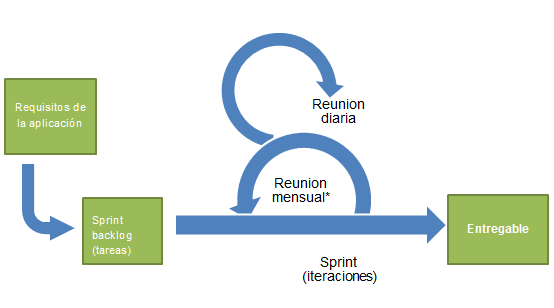
\includegraphics[width=0.7\linewidth]{./Figures/Scrumm.PNG}
    \caption[Proceso iterativo Scrum]{En este gráfico podemos ver el método de trabajo según Scrum, en el cual se observa lo importante que son los entregables}
    \label{fig:Scrum}
\end{figure}



%\newpage
Scrum, de manera resumida consiste en lo siguiente:
\begin{enumerate}
    \item Hablar con el cliente para ver si hay nuevos requisitos.
    \item Crear backlog, es decir, las tareas de ese sprint.
    \item Programar los requisitos especificados en el sprint.
    \item Reunión de retrospectiva para ver que ha ido mal y mejorarlo.
    \item Enviar entregable al cliente.
    \item Repetir.
\end{enumerate}

Es fundamental entre sprint y sprint que el valor del producto haya aumentado. Es decir, lo importante es el producto, no como vamos nosotros en el propio proyecto. Podríamos haber avanzado mucho en el diseño del software, pero si eso es algo que el cliente no puede ver estaremos fallando en nuestra agilidad.

Por otro lado, si cometemos algún error será muy sencillo corregir el error ya que si los sprints son de dos semanas por ejemplo, no habremos perdido apenas tiempo. Y además para el cliente los entregables serán predecibles en el tiempo.

Scrum es también muy importante, y se posiciona como una alternativa muy potente frente a COCOMO o waterfall, es porque en la creación de software hay un componente de incertidumbre muy grande. No sabemos como, ni cuando pueden cambiar los requisitos de un software. Por ello toman importancia los sprints de nuevo. 

En los modelos antiguos, si ya habíamos terminado la fase de análisis y diseño, y se requería una nueva funcionalidad es necesario paralizar el desarrollo del software y volver a analizar y diseñar. En cambio, con Scrum es posible integrar ese cambio en el siguiente sprint.

\subsection{Kanban}
Kanban es un método de organización del conocimiento del trabajo que se está realizando con un gran énfasis en el la entrega justo a tiempo \footnote{JIT Delivery: Just-In-Time Delivery} sin sobrecargar al equipo \cite{Kanban:WhatIsIt}.

Kanban se centra mucho en que lo importante no es empezar muchas cosas, si no que acabemos aquello que empezamos. Sirve sobre todo para ver de una manera visual:
\begin{itemize}
    \item Qué tenemos pendiente
    \item Qué estamos haciendo ahora mismo
    \item Qué hemos terminado.
\end{itemize}

El m\'{e}todo Kanban es algo muy extenso, pero yo simplemente he aplicado el tablero Kanban mezclado con Scrum. 
Cada dos semanas, me creo una lista de tareas que debo completar (Backlog) y lo coloco en la columna de ``Tareas pendientes´´, 
ordenadas por prioridad. Después, coloco en la lista de ``En progreso´´ como m\'{a}ximo dos tareas. Y no empiezo ninguna otra hasta 
que esas dos hayan sido pasadas a la columna de ``Tareas finalizadas´´.

\subsection{Mi planificaci\'{o}n}
Cada sprint tiene una duraci\'{o}n de un mes, empezando desde Septiembre del 2013.
\subsubsection{Sprint 1}
Este sprint era el comienzo del proyecto, establecer prioridades, documentarse etc. Lo que ha compuesto este sprint ha sido:

\begin{itemize}
    \item Crear y configurar el repositorio Git y los clientes en los dos ordenadores.
    \item Leer la documentaci\'{o}n existente y obtener el c\'{o}digo fuente original.
    \item Iniciar dise\~{n}os gr\'{a}ficos preliminares en papel para elegir las librer\'{i}as necesarias.
    \item Buscar y documentarse sobre las librer\'{i}as que cumplan los requisitos del punto anterior. 
\end{itemize} 

\subsubsection{Sprint 2}
Una vez configurado y elegidas las librer\'{a}s necesarias:

\begin{itemize}
    \item Reunirse con Mikel para realizar una captura de requisitos.
    \item Dise\~{n}ar unos prototipos funcionales.
    \item Documentar lo que se hab\'{i}a realizado hasta el momento, es decir, el tipo de planificaci\'{o}n que se hab\'{i}a elegido,
    tecnolog\'{i}as que se iban a usar etc.
\end{itemize}

\subsubsection{Sprint 3}
El siguiente paso consiste en poder cargar v\'{i}deos, tantos como se quieran, desde el sistema de archivos.

\begin{itemize}
    \item Crear el control de cargar v\'{i}deos (contenedor de v\'{i}deos). El contenedor debe permitir:
    \begin{itemize}
        \item Cargar distintos v\'{i}deos desde el sistema de archivos.
        \item Cada v\'{i}deo debe disponer de sus controles individuales. Play, pausa, stop y avanzar de tantos segundos en tantos segundos, y que sea
        configurable por el usuario, mediante un archivo de configuraci\'{o}n.
        \item El contenedor de v\'{i}deos debe disponer de unos controles generales que pause, y que los reproduzca de manera simult\'anea
        para mantener la sincronizaci\'{o}n.
        \item Debe permitir establecer para cada v\'{i}deo el momento de inicio del v\'{i}deo manualmente para mantener la sincronizaci\'{o}n.
    \end{itemize}
\end{itemize}

\subsubsection{Sprint 4}
Despu\'{e}s de terminar la visualizaci\'{o}n de v\'{i}deos, lo siguiente en la lista de tareas es crear un visualizador de datos.

\begin{itemize}
    \item Crear el contenedor que nos permita ver datos. El control debe permitir:
    \begin{itemize}
        \item Visualizar datos continuos y discretos.
        \item Seleccionar un rango en la gr\'{a}fica, estableciendo un inicio y un fin para las propiedades.
        \item Que muestre el progreso, y que este sincronizado con el v\'{i}deo.
        \item Guardar el inicio y fin seleccionado.
    \end{itemize}
\end{itemize}

\subsubsection{Sprint 5}
Ya tenemos todo preparado para funcionar, ahora hay que poder guardar datos.

\begin{itemize}
    \item Elegir el m\'etodo de guardado de los datos.
    \item Configurar la base de datos (si aplica).
    \item Crear el diagrama Entidad-Relaci\'{o}n que representara el modo de guardado de datos (si aplica).
    \item A\~{n}adir al c\'{o}digo existente las llamadas necesarias a la base de datos (si aplica).
    \item Permitir cambiar la ubicaci\'{o}n de la base de datos mediante un archivo de configuraci\'{o}n (Si aplica).
\end{itemize}

\subsubsection{Sprint 6}
En este momento ya tenemos una aplicaci\'{o}n completamente funcional pero con datos de prueba. Hay que poder cargar datos de los XML.

\begin{itemize}
    \item Crear la clase para interactuar con los XML.
    \item Hablar con Mikel para saber como est\'{a}n guardadas las observaciones.
    \item Utilizando los datos del XML cargar la aplicaci\'{o}n con esos datos.
\end{itemize}

\section{Herramientas}
El proyecto, al no ser enteramente m\'io, no he tenido una libertad total para la elecci\'on de herramientas. 

Las herramientas que he utilizado para llevar a cabo este proyecto han sido:
\begin{itemize}
    \item 
    \textbf{Visual Studio}
    
    Para el desarrollo propiamente dicho del proyecto he usado Visual Studio 2013 Ultimate, proporcionado de manera gratuita gracias al acuerdo que mantiene la UPV/EHU con Microsoft.
    
    \item 
    \textbf{TeXstudio y \LaTeX}
    
    Dos herramientas gratuitas y de código abierto para generar documentos.
    
    \item
    \textbf{Git y GitHub}
    
    Fundamental en los proyectos que se basen en metodologías ágiles. Git es un software de gestión de control de versiones distribuido, esto es, que cada desarrollador dispone de una copia completa del repositorio, desarrollado por Linus Torvalds y Junio Hamano en 2005 y similar a SVN.
    
    \item
    \textbf{OxyPlot}
    
    Librer\'{i}a de c\'{o}digo abierto y multiplataforma que permite crear gr\'{a}ficos de manera sencilla as\'{i} como seleccionar rangos etc.
    
\end{itemize}

\section{Gesti\'{o}n de riesgos}
Dadas las fechas de entrega impuestas por mi mismo para la finalizaci\'{o}n del Trabajo de Fin de Grado, es un hecho que
aparecerán riesgos que pueden poner en peligro el proyecto. Es por ello que se necesita tener en cuenta las probabilidades de los sucesos que 
pueden ocurrir y que puedan retrasar el trabajo de forma notable. Una vez
listados, se puede proceder a crear un plan de prevención para evitarlos. Y en caso de que la prevención no
funcionara, un plan de contingencia que pueda amortiguar las consecuencias de ese riesgo. A continuación
se listan de forma detallada los riesgos que pueden aparecer durante el transcurso del proyecto.

\subsection{Planificaci\'{o}n}
En esta categor\'{i}a se engloban los riesgos que sean causados por una mala planificaci\'{o}n temporal.
\subsubsection{Mala concepci\'{o}n del proyecto}
\begin{table}[H]
    \begin{center}
       \rowcolors{1}{lightgray}{} %\rowcolors{<starting row index>}{<odd row color>}{<even row color>}
       \begin{tabular}{l p{8cm}}
           Descripci\'{o}n                 & Por decisiones erróneas, como puede ser elegir utilizar una
           base de datos, puede que el trabajo deba ser reconstruido desde el principio. \\
           Prevenci\'{o}n                  & Una buena planificación y conocimiento exacto de lo que quiere y necesita el cliente. \\ 
           Plan de contingencia            & Un programa flexible a cambios \\
           Probabilidad                    & Improbable \\
           Impacto                         & Muy alto\\
        \end{tabular}
    \end{center}
    
\end{table}
\subsubsection{Error en la planificaci\'{o}n temporal}
\begin{table}[H]
    \begin{center}
        \rowcolors{1}{lightgray}{} %\rowcolors{<starting row index>}{<odd row color>}{<even row color>}
        \begin{tabular}{l p{8cm}}
            Descripci\'{o}n                 & Por una mala compresión y falta de experiencia el cálculo
            de tiempo estimado de una de las tareas es erróneo y hay que reajustar todo el proyecto. \\
            Prevenci\'{o}n                  & Realizar la estimación lo mejor posible y tener una buena
            comunicación con el cliente para no tener fallos de comprensión. \\ 
            Plan de contingencia            & Margen de error en los tiempos \\
            Probabilidad                    & Muy probable \\
            Impacto                         & Medio\\
        \end{tabular}
    \end{center}
    
\end{table}
\subsection{Entorno de desarrollo}
\subsubsection{Incompatibilidad de versiones}
\begin{table}[H]
    \begin{center}
        \rowcolors{1}{lightgray}{} %\rowcolors{<starting row index>}{<odd row color>}{<even row color>}
        \begin{tabular}{l p{8cm}}
            Descripci\'{o}n                 & Al utilizar dos ordenadores, una workstation y un port\'{a}til puede que no disponga de las mismas
            versiones del software o que no se satisfagan todas las dependencias. \\
            Prevenci\'{o}n                  & Asegurarme de disponer el mismo software con las mismas versiones. \\ 
            Plan de contingencia            & Resolver manualmente las dependencias. \\
            Probabilidad                    & Probable \\
            Impacto                         & Bajo\\
        \end{tabular}
    \end{center}
    
\end{table}
\subsubsection{Problemas con GIT}
\begin{table}[H]
    \begin{center}
        \rowcolors{1}{lightgray}{} %\rowcolors{<starting row index>}{<odd row color>}{<even row color>}
        \begin{tabular}{l p{8cm}}
            Descripci\'{o}n                 & Al ser algo no ense\~{n}ado en profundidad en clase puede causar problemas al usar las
            funciones avanzadas. \\
            Prevenci\'{o}n                  & Tener un buen manual y tener una copia local en otra carpeta para prevenir perdidas de informaci\'{o}n. \\ 
            Plan de contingencia            & Desechar el software de control de versiones y buscar alternativas como Dropbox. \\
            Probabilidad                    & Poco probable \\
            Impacto                         & Bajo \\
        \end{tabular}
    \end{center}  
\end{table}
\subsubsection{Problemas con las librer\'{i}as}
\begin{table}[H]
    \begin{center}
        \rowcolors{1}{lightgray}{} %\rowcolors{<starting row index>}{<odd row color>}{<even row color>}
        \begin{tabular}{l p{8cm}}
            Descripci\'{o}n                 & Que las librar\'{i}as escogidas no cumplan los requisitos necesarios \\
            Prevenci\'{o}n                  & Mirar con anterioridad que las librar\'{i}as cumplen todos nuestros requisitos. \\ 
            Plan de contingencia            & Buscar otra librar\'{i}a o intentar parchear la actual, ya que son de c\'{o}digo abierto. \\
            Probabilidad                    & Muy probable \\
            Impacto                         & Alto \\
        \end{tabular}
    \end{center}
    
\end{table}
\subsection{Usuarios finales y clientes}
\subsubsection{No agrado del producto}
\begin{table}[H]
    \begin{center}
        \rowcolors{1}{lightgray}{} %\rowcolors{<starting row index>}{<odd row color>}{<even row color>}
        \begin{tabular}{l p{8cm}}
            Descripci\'{o}n                 & Despu\'{e}s de la entrega del proyecto puede suceder que el cliente no est\'{e} satisfecho. \\
            Prevenci\'{o}n                  & Una buena comunicación con el cliente y reuniones progresivas para ir mostrando la evolución del proyecto. \\ 
            Plan de contingencia            & Blindar las caracter\'{i}sticas, solo se realizaran las estipuladas durante el proyecto. \\
            Probabilidad                    & Probable \\
            Impacto                         & Muy alto \\
        \end{tabular}
    \end{center}
    
\end{table}

\subsubsection{Manejo poco intuitivo}
\begin{table}[H]
    \begin{center}
        \rowcolors{1}{lightgray}{} %\rowcolors{<starting row index>}{<odd row color>}{<even row color>}
        \begin{tabular}{l p{8cm}}
            Descripci\'{o}n                 & Como  los  programadores  tienen  un  conocimiento
            inform\'{a}tico superior no tendr\'{a}n problemas con el uso, pero los usuarios si pueden tenerlos.\\
            Prevenci\'{o}n                  & Un diseño de interfaz sencillo y probar versiones con
            usuarios con conocimientos inform\'{a}ticos bajos. \\ 
            Plan de contingencia            & Adaptar la interfaz en el siguiente sprint. \\
            Probabilidad                    & Probable. \\
            Impacto                         & Alto \\
        \end{tabular}
    \end{center}
    
\end{table}

\subsection{Personas}
\subsubsection{Bajas por enfermedad}
\begin{table}[H]
    \begin{center}
        \rowcolors{1}{lightgray}{} %\rowcolors{<starting row index>}{<odd row color>}{<even row color>}
        \begin{tabular}{l p{8cm}}
            Descripci\'{o}n                 & El \'{u}nico componente del equipo cae enfermo y no puede trabajar. \\
            Prevenci\'{o}n                  & No existe prevenci\'{o}n. \\ 
            Plan de contingencia            & Recuperarse lo antes posible y manejar cierta holgura con las fechas.\\
            Probabilidad                    & Probable. \\
            Impacto                         & Muy alto \\
        \end{tabular}
    \end{center}
    
\end{table}

\subsection{Requisitos}
\subsubsection{Nuevos requisitos}
\begin{table}[H]
    \begin{center}
        \rowcolors{1}{lightgray}{} %\rowcolors{<starting row index>}{<odd row color>}{<even row color>}
        \begin{tabular}{l p{8cm}}
            Descripci\'{o}n                 & Debido a que el cliente tiene nuevas necesidades solicita la
            implementaci\'{o}n de funcionalidades extras o la desaparici\'{o}n de alguna que se hayan podido volver innecesarias. \\
            Prevenci\'{o}n                  & Realizar un buen dise\~{n}o para la posibilidad de añadir
            funcionalidades sin que suponga un coste muy elevado. \\ 
            Plan de contingencia            & Evaluar los nuevos requisitos para saber si se pueden
            abordar o no y si fuese que si estudiar la situación y asignar el trabajo a los trabajadores. \\
            Probabilidad                    & Probable \\
            Impacto                         & Alto \\
        \end{tabular}
    \end{center}
    
\end{table}

\subsubsection{Requisitos no contemplados (ocultos)}
\begin{table}[H]
    \begin{center}
        \rowcolors{1}{lightgray}{} %\rowcolors{<starting row index>}{<odd row color>}{<even row color>}
        \begin{tabular}{l p{8cm}}
            Descripci\'{o}n                 & Requisitos explícitos desde el principio, pero que no fueron
            vistos en el primer an\'{a}lisis y al verlos en un futuro, provocan cambios en todos los niveles. \\
            Prevenci\'{o}n                  & Utilizar correctamente Scrum. \\ 
            Plan de contingencia            & A\~{n}adirlo como una tarea al siguiente sprint. \\
            Probabilidad                    & Muy probable. \\
            Impacto                         & Medio-Bajo. \\
        \end{tabular}
    \end{center}
    
\end{table}

\section{Planificaci\'{o}n econ\'{o}mica}
No se obtendr\'{a} beneficio econ\'{o}mico del proyecto ya que se hace por el bien de la ciencia, y porque esta licenciado
bajo licencia GPLv3.

Por lo tanto el coste de venta de nuestro coste sera 0€

\subsection{Amortizaci\'{o}n de material}
\subsubsection{Oficina}
La oficina que utilizamos es el domicilio familiar y no hay que pagar alquiler ya que es de nuestra propiedad. Por lo que el gasto de alquiler/hipoteca es 0€
\subsubsection{Material inform\'{a}tico}
El material informático que se va a usar es un portátil Acer TravelMate 5742G comprado en 
Diciembre de 2010 y usado intensivamente durante estos 4 años. 
El portátil estaba pensado para ser amortizado en 4 años. \emph{As\'{i} que por aqui habra que hacer algun calculo tonto}, por lo que durante el 
transcurso del TFG no va a generar ning\'{u}n tipo de gasto, ni beneficio, porque recordemos, es un proyecto sin \'{a}nimo de lucro.

Tambi\'{e}n se va a usar un PC gen\'{e}rico comprado a piezas en 2012.


\subsection{Otros gastos}

\begin{tabular}{l*{1}{c}r}
    Concepto                   & Gastos en € / mes & \\
    \hline
    Luz                        & 60 & \\
    Agua                       & 50 & \\
    Internet + Teléfono        & 60 & \\
    Gas                        & 70 & \\
    \hline
    Total Mes                  & 325 & \\
    Total A\~{n}o              & 3900 &\\
\end{tabular}

